\chapter*{Experiment 5 - Phenakistoscope Creation}
\addcontentsline{toc}{chapter}{Experiment 5 - Phenakistoscope Creation}
We wire up the experiment as shown in the diagram fig:~\ref{fig:exp4_mp3}. And upload the sketch code in the next section on page:~\pageref{sketch:exp4}.

%
\begin{figure}[ht]
	\centering
	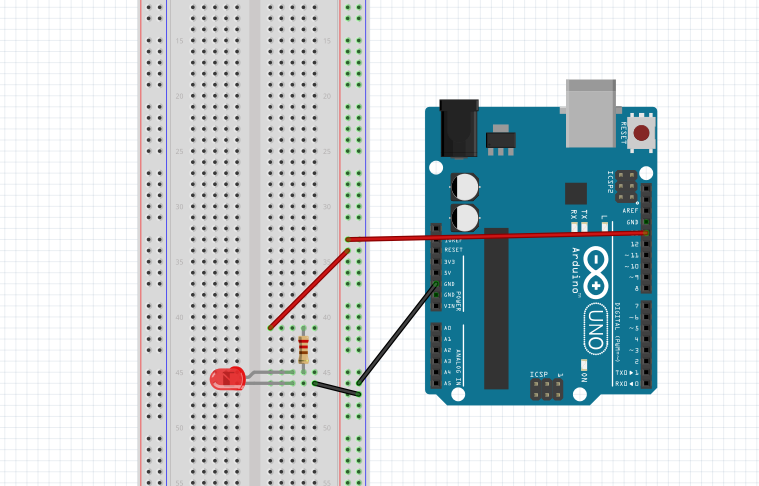
\includegraphics[width=12cm]{images/07}
	\caption{LED Phenakistoscope \citep{fritzing-15}}
	\label{fig:exp5_phenakistoscope}
\end{figure}
%

When the Arduino boots, the led should flash on for a second, then off for a second and repeat.


%
\begin{figure}
	\centering
	\begin{subfigure}[t]{5cm}
		\centering
		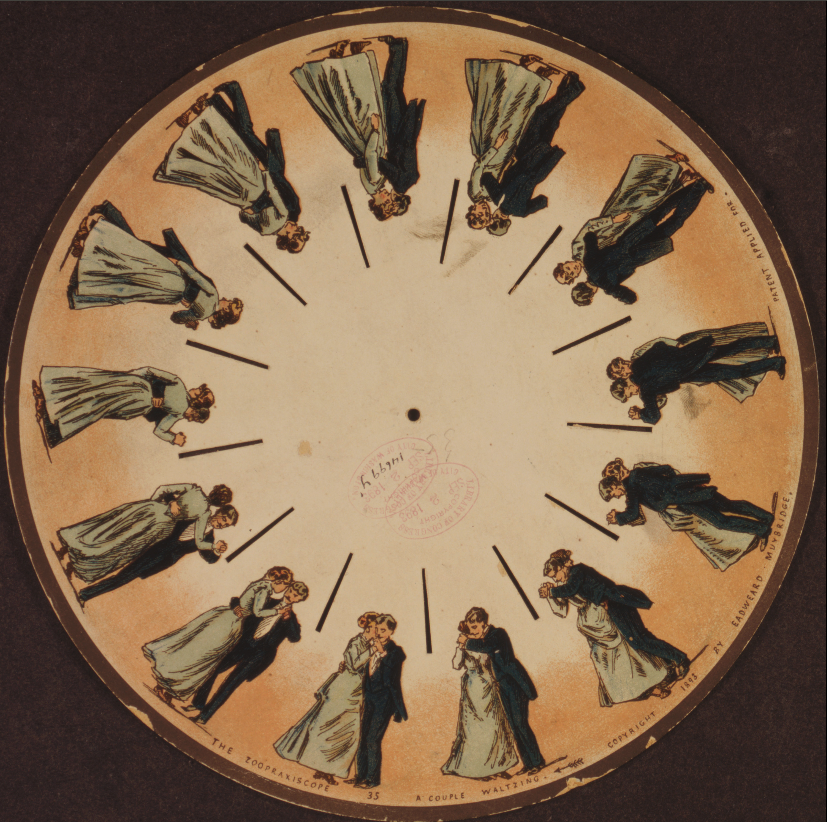
\includegraphics[width=5cm]{images/12}
		\caption{A couple waltzing - Eadweard Muybridge, 1893}
		\label{fig:gqrx_spectrogram_01} 
	\end{subfigure}
	\quad
	\begin{subfigure}[t]{5cm}
		\centering
		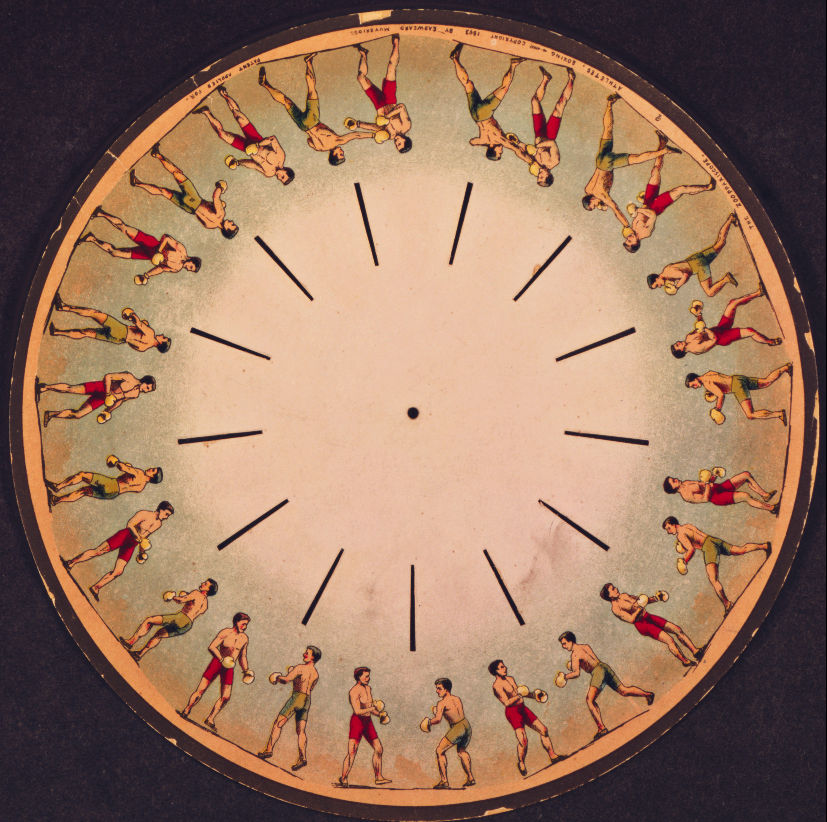
\includegraphics[width=5cm]{images/13}
		\caption{Athletes Boxing - Eadweard Muybridge, 1890}
		\label{fig:rtl_power_spectrogram_01} 
	\end{subfigure}
	\quad
	\begin{subfigure}[t]{5cm}
		\centering
		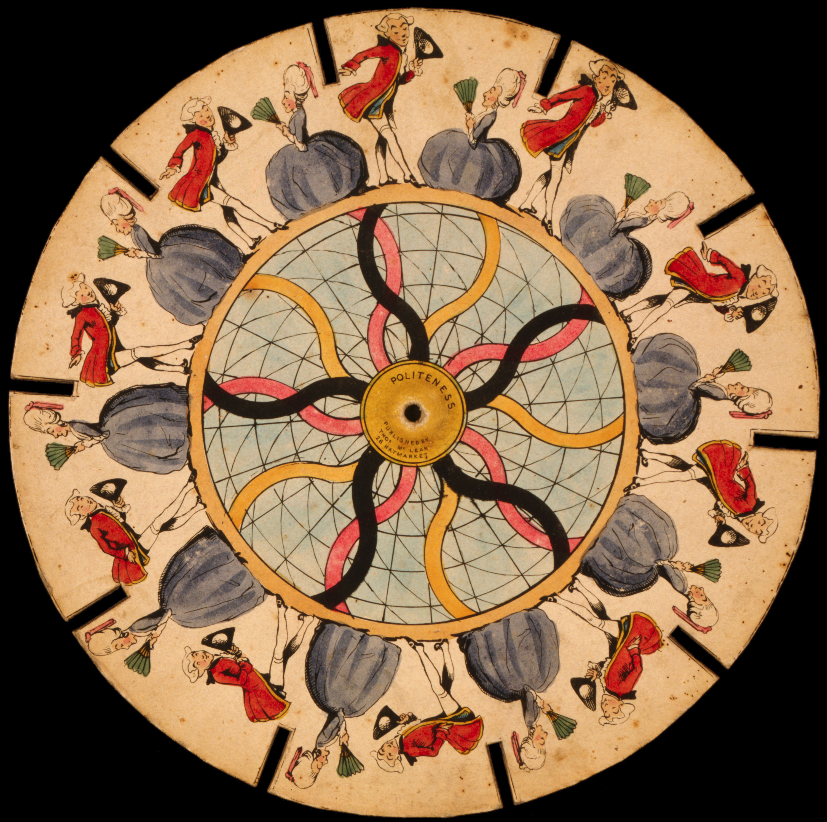
\includegraphics[width=5cm]{images/14}
		\caption{Politeness - Thos. McLean, 1833}
		\label{fig:rtl_power_spectrogram_02} 
	\end{subfigure}
	\quad
	\begin{subfigure}[t]{5cm}
		\centering
		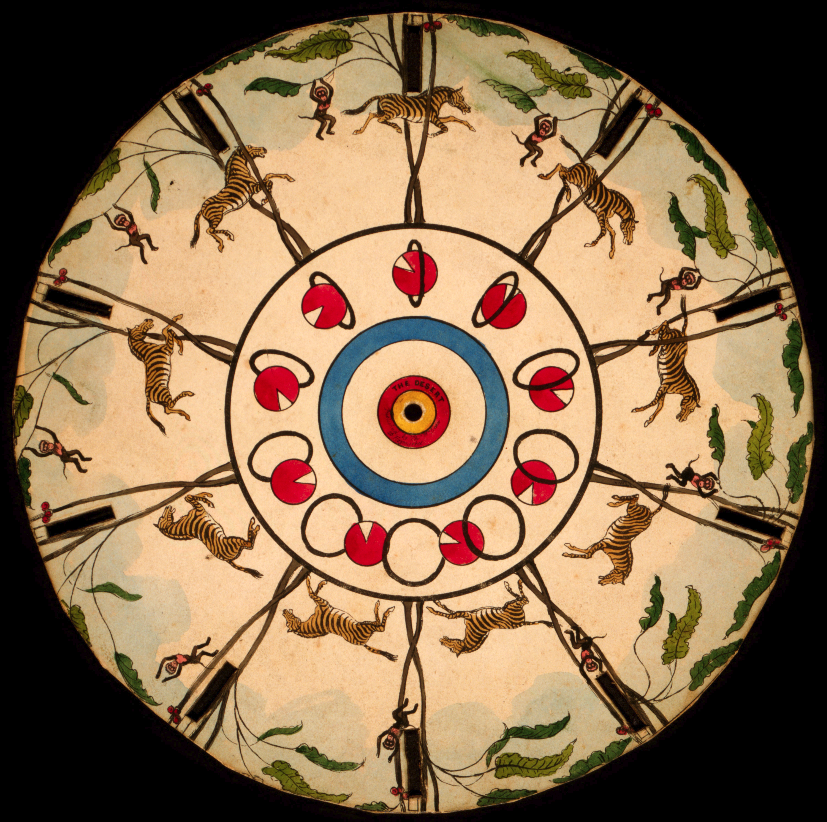
\includegraphics[width=5cm]{images/15}
		\caption{The Desert - Thos. McLean, 1833}
		\label{fig:rtl_power_spectrogram_03} 
	\end{subfigure}
	\quad
	\caption{A selection of Phenakistoscopes}
	\label{fig:phenakistoscopes}
\end{figure}
%


\newpage
\section*{Sketch Code}
\label{sketch:exp5}
\begin{lstlisting}
/*
Blink
Turns on an LED on for one second, then off for one second, repeatedly.

This example code is in the public domain.
*/

// the setup function runs once when you press reset or power the board
void setup() {
  // initialize digital pin 13 as an output.
  pinMode(13, OUTPUT);
}

// the loop function runs over and over again forever
void loop() {
  // turn the LED on 
  // (HIGH is the voltage level)
  digitalWrite(13, HIGH);
	
  //wait for 1000 milliseconds
  delay(1000);
	
  // turn the LED off by making 
  // the voltage LOW
  digitalWrite(13, LOW);    
	            
  // wait for 1000 milliseconds              
  delay(1000);
}
\end{lstlisting}
\citep{kalif-15-a} \citep{kalif-15-b} \cite{pepi-11}